\documentclass[12pt,]{article}
\usepackage{lmodern}
\usepackage{amssymb,amsmath}
\usepackage{ifxetex,ifluatex}
\usepackage{fixltx2e} % provides \textsubscript
\ifnum 0\ifxetex 1\fi\ifluatex 1\fi=0 % if pdftex
  \usepackage[T1]{fontenc}
  \usepackage[utf8]{inputenc}
\else % if luatex or xelatex
  \ifxetex
    \usepackage{mathspec}
  \else
    \usepackage{fontspec}
  \fi
  \defaultfontfeatures{Ligatures=TeX,Scale=MatchLowercase}
\fi
% use upquote if available, for straight quotes in verbatim environments
\IfFileExists{upquote.sty}{\usepackage{upquote}}{}
% use microtype if available
\IfFileExists{microtype.sty}{%
\usepackage{microtype}
\UseMicrotypeSet[protrusion]{basicmath} % disable protrusion for tt fonts
}{}
\usepackage[margin=1in]{geometry}
\usepackage{hyperref}
\hypersetup{unicode=true,
            pdfborder={0 0 0},
            breaklinks=true}
\urlstyle{same}  % don't use monospace font for urls
\usepackage{graphicx,grffile}
\makeatletter
\def\maxwidth{\ifdim\Gin@nat@width>\linewidth\linewidth\else\Gin@nat@width\fi}
\def\maxheight{\ifdim\Gin@nat@height>\textheight\textheight\else\Gin@nat@height\fi}
\makeatother
% Scale images if necessary, so that they will not overflow the page
% margins by default, and it is still possible to overwrite the defaults
% using explicit options in \includegraphics[width, height, ...]{}
\setkeys{Gin}{width=\maxwidth,height=\maxheight,keepaspectratio}
\IfFileExists{parskip.sty}{%
\usepackage{parskip}
}{% else
\setlength{\parindent}{0pt}
\setlength{\parskip}{6pt plus 2pt minus 1pt}
}
\setlength{\emergencystretch}{3em}  % prevent overfull lines
\providecommand{\tightlist}{%
  \setlength{\itemsep}{0pt}\setlength{\parskip}{0pt}}
\setcounter{secnumdepth}{0}
% Redefines (sub)paragraphs to behave more like sections
\ifx\paragraph\undefined\else
\let\oldparagraph\paragraph
\renewcommand{\paragraph}[1]{\oldparagraph{#1}\mbox{}}
\fi
\ifx\subparagraph\undefined\else
\let\oldsubparagraph\subparagraph
\renewcommand{\subparagraph}[1]{\oldsubparagraph{#1}\mbox{}}
\fi

%%% Use protect on footnotes to avoid problems with footnotes in titles
\let\rmarkdownfootnote\footnote%
\def\footnote{\protect\rmarkdownfootnote}

%%% Change title format to be more compact
\usepackage{titling}

% Create subtitle command for use in maketitle
\providecommand{\subtitle}[1]{
  \posttitle{
    \begin{center}\large#1\end{center}
    }
}

\setlength{\droptitle}{-2em}

  \title{}
    \pretitle{\vspace{\droptitle}}
  \posttitle{}
    \author{}
    \preauthor{}\postauthor{}
    \date{}
    \predate{}\postdate{}
  
\usepackage{pdflscape}
\newcommand{\blandscape}{\begin{landscape}}
\newcommand{\elandscape}{\end{landscape}}

\begin{document}

\hypertarget{habitat-and-fishing-control-grazing-potential-on-coral-reefs}{%
\subsection{Habitat and fishing control grazing potential on coral
reefs}\label{habitat-and-fishing-control-grazing-potential-on-coral-reefs}}

James PW Robinson, Jamie M McDevitt-Irwin, Jan-Claas Dajka, Jeneen
Hadj-Hammou, Samantha Howlett, Alexia Graba-Landry, Andrew S Hoey,
Kirsty L Nash, Shaun K Wilson, Nicholas AJ Graham

\hypertarget{supplementary-methods}{%
\paragraph{Supplementary Methods}\label{supplementary-methods}}

\emph{Region details}

In Seychelles, 21 reefs were surveyed in 2008, 2014, and 2017 on two
inhabited islands (Mahe, Praslin). Surveys were conducted on the reef
slope at 9-12 m depth, and stratified to include carbonate fringing
reefs, granitic rocky reefs with coral growth, and patch reef habitats
on a sand, rubble, or rock base (Fig. S1B). Surveys were repeated for
either 8 (2008) or 16 (2011, 2014, 2017) replicates at each reef, which
were located at least 15 m away from each other. To ensure that survey
effort was comparable among Seychelles reefs, we only considered surveys
from the first 8 replicates (per site per survey year). Overall, the
surveys covered up to 0.5 km of reef front and 2,500
m\textsuperscript{2} of reef habitat, including 672 point counts over 4
surveyed years. Reefs were categorised by their exploitation status,
with 9 sites in small protected areas and 12 sites supporting artisanal
fisheries.

In the Chagos archipelago, 25 reefs were surveyed on four uninhabited
atolls in 2010 (Fig. S1B). Surveys were stratified to include sheltered
(9) and exposed (9) habitats, and four replicate transects were
conducted at each site, resulting in 100 total transects. All reefs were
categorised as remote.

In Maldives, 11 reefs were surveyed on one atoll (Huvadhoo) in 2013
(Fig. S1B). Surveys were conducted on the reef slope for 4 replicates
per reef, resulting in 44 total transects. All reefs were categorised as
fished.

In Australia, five reefs were surveyed on the central Great Barrier Reef
in 2010 and 2011 (Wheeler, Davies, Rib, Trunk, John Brewer) (Graham et
al.~2014) (Fig. S1B). Reefs were stratified to include 3 wave exposed
and 3 wave sheltered locations (6 per reef), which were further divided
into reef slope (7-9 m depth), reef crest (2-3 m depth), and reef flat
(100 m distance from crest). Each location and habitat type was surveyed
with four replicate transects. We used data for surveys conducted on the
reef slope, which produced a dataset of 24 transects per reef and 120
transects in total. Davies, Rib, Trunk and John Brewer were categorised
as fished, and Wheeler was categorised as protected (no-take zone).

\emph{Benthic categories}

To understand the range of benthic habitat types across the dataset, we
categorised reefs according to their benthic regime, using a
correlation-based PCA and K-means clustering (Jouffray et al.~2015). The
optimal number of clusters was found using an elbow method with k = 2-15
range, and then applied to the K-means clustering. For reefs in
Seychelles which were surveyed in multiple years, we estimated regimes
at each site by averaging cover values over time. Across all reefs, we
detected three benthic regimes characterised by 1) hard coral dominance,
2) high availability of bare substrate, and 3) rubble reefs (Fig. S1B).
Coral dominance was the most common regime, detected at 53 reefs across
all four regions, whereas bare substrate regimes were only present in
Seychelles (14) and Chagos (7). Rubble reefs were only present in
Seychelles (6 reefs).

\emph{Bite rate models}

Cropper function was quantified in terms of potential feeding intensity,
the total number of bites per minute, and derived from a predictive
model which accounted for species- and genera-specific bite rates (Eqs.
1,2). In our cropper feeding data, bite rates were only weakly
correlated with TL (Pearson's r = -0.18), and so we assumed bite rates
were unrelated to body size.

\(biterate = Gamma(\mu, \theta)\) \hfill Eq. 1

\(log(\mu) = \beta_0 + species_i + genus_j + dataset_k\) \hfill Eq. 2

From this model, we generated species- and genera-level posterior
predictions of grazing rates and assigned to each individual cropping
fish observed in UVCs. Fish belonging to genera which were not present
in the feeding observation dataset were assigned average feeding rates
irrespective of species and genera (i.e.~the model intercept,
\texttt{\textbackslash{}beta\_0}). Following Van Rooij et al. (1998),
daily carbon intake was linked to body mass (M, grams) as

\(gC = 0.0342.M^{0.816}\) \hfill Eq.3

which we then divided by the predicted number of bites per day to
produce an estimate of grams carbon consumed per minute by each
individual cropping fish. Our approach accounts for bite size increasing
with body size, meaning that larger fish will have greater carbon
intakes (Marshell \& Mumby 2015). We summed estimates within UVC
replicates (i.e.~point count or transect) and averaged across replicates
to give site-level estimates of potential cropping function.

Scraping function was quantified terms of potential area of substrata
cleared per minute. Feeding observations provided estimates of bite
rates, which we modelled as a function of body size (TL, cm; \emph{r} =
-0.43) according to species- and genera-specific grazing rates, for
gamma distributed errors (Eqs. 4, 5).

\(biterate = Gamma(\mu, \theta)\) \hfill Eq. 4

\(log(\mu) = \beta_0 + \beta_1*TL + species_i + genus_j + dataset_k\)
\hfill Eq. 5

To account for potential differences in scraping action among species
and across body sizes, we used a second underwater feeding observation
dataset of scraper bite areas. Bite scar area (cm\textsuperscript{2})
was modelled as a function of body size (TL, cm; \emph{r} = 0.83), for
Gamma distributed errors (Eqs. 6,7).

\(scarsize = Gamma(\mu, \theta)\) \hfill Eq. 6

\(log(\mu) = \beta_0 + \beta_1*TL\) \hfill Eq. 7

By including size (TL) as an explanatory covariate, models accounted for
scar area increasing with body size (Fig. S2A) and bite rates decreasing
with body size (Fig. S2B). For each observed scraper in the UVC dataset,
we generated posterior predictions for bite rate and scar size according
to its species identity and body size. Species which were not observed
in feeding observations were assigned genera-level bite rates. These
predictions were converted to area scraped per minute (bite rate x scar
size = area scraped) (m\textsuperscript{2} ha\textsuperscript{-1}
min\textsuperscript{-1}), summed within surveys and averaged to give
site-level estimates of potential scraping function.

All models fitted to feeding data were fitted with weakly informative
priors (Table S2) using Markov Chain Monte Carlo sampling implemented in
Stan. We sampled three chains of 3,000 iterations (warmup = 1,500) each
for model checks, and one long chain of 5,000 iterations (warmup =1,500)
for generating grazing predictions. Model convergence was assessed by
inspecting posterior predictions, Gelman-Rubin diagnostic (Rhat), and
the number of effective samples (Table S2).

~

\hypertarget{references}{%
\paragraph{References}\label{references}}

Graham, N. A. J., Chong-Seng, K. M., Huchery, C., Januchowski-Hartley,
F. A., \& Nash, K. L. (2014). Coral reef community composition in the
context of disturbance history on the Great Barrier Reef, Australia.
PloS One, 9(7), e101204.

Jouffray, J.-B., Nyström, M., Norström, A. V., Williams, I. D., Wedding,
L. M., Kittinger, J. N., \& Williams, G. J. (2015). Identifying multiple
coral reef regimes and their drivers across the Hawaiian archipelago.
Proceedings of the Royal Society B: Biological Sciences, 370(1659),
20130268.

Marshell, A., \& Mumby, P. J. (2015). The role of surgeonfish
(Acanthuridae) in maintaining algal turf biomass on coral reefs. Journal
of Experimental Marine Biology and Ecology, 473, 152--160.

Van Rooij, J. M., Videler, J. J., \& Bruggemann, J. H. (1998). High
biomass and production but low energy transfer effciency of Caribbean
parrotfish: implications for trophic models of coral reefs. Journal of
Fish Biology, 53(sA), 154--178.

\begin{center}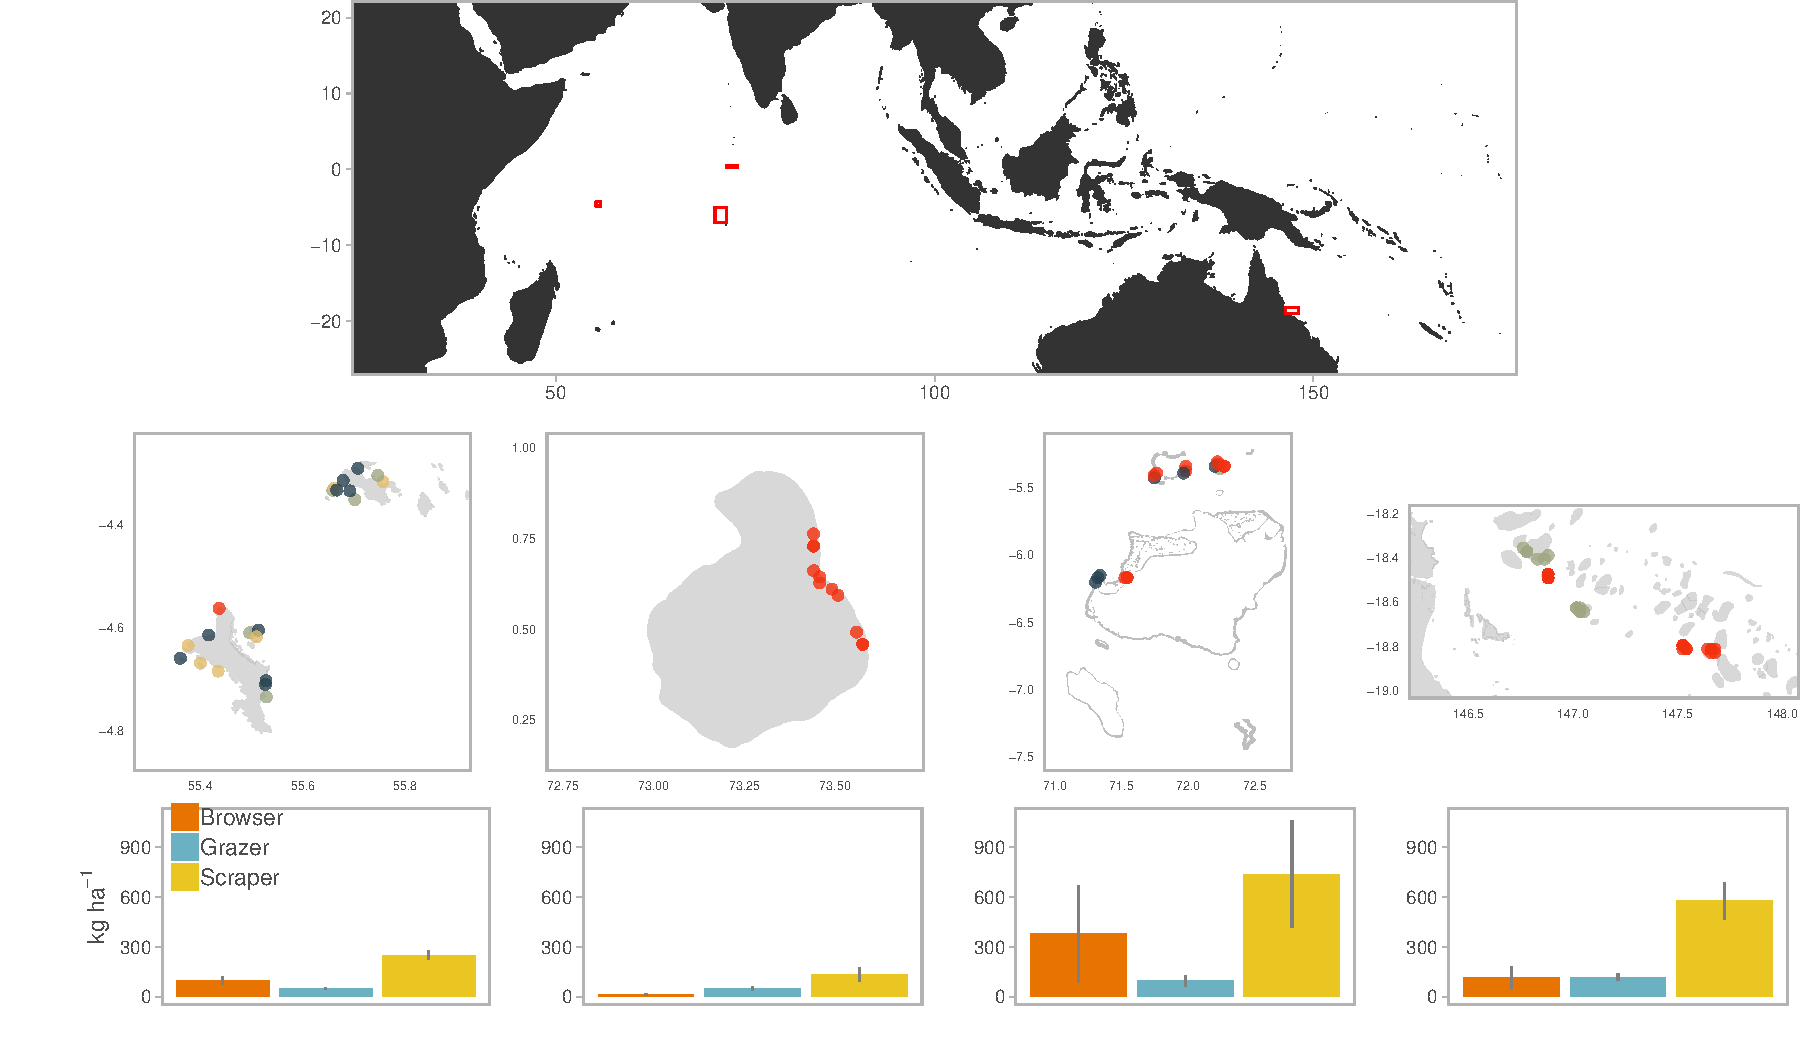
\includegraphics[width=480px]{../../figures/Figure1} \end{center}

\textbf{Figure S1 \textbar{} Map of study sites with benthic habitat
regimes (B) and herbivore biomass levels (C).} Survey sites are coloured
by regimes identified in k-cluster analysis (coral = blue, substrate =
red, rubble = yellow), and bar plots show mean grazing biomass (± 2
standard errors) for croppers and scrapers.

\newpage

\begin{center}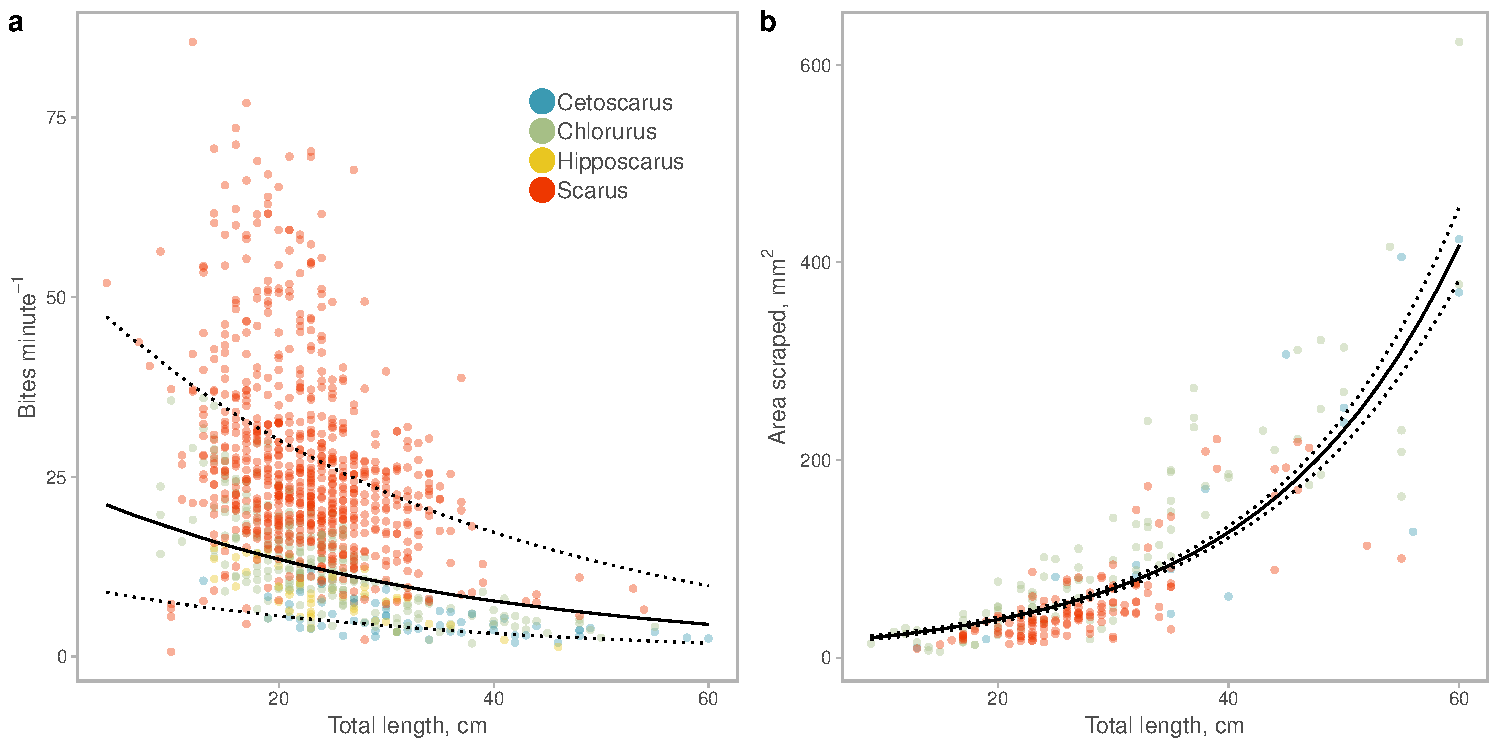
\includegraphics[width=480px]{../../figures/FigureS1_scrape_size} \end{center}

\textbf{Figure S2 \textbar{} Size effects on scraper bite rates (A) and
bite area (B).} Lines indicate median posterior predictions with 95\%
certainty intervals, excluding species and genera effects, across the
range of observed body sizes (total length, cm). Points are observed
bite rates or bite areas coloured by genera.

\newpage

\begin{center}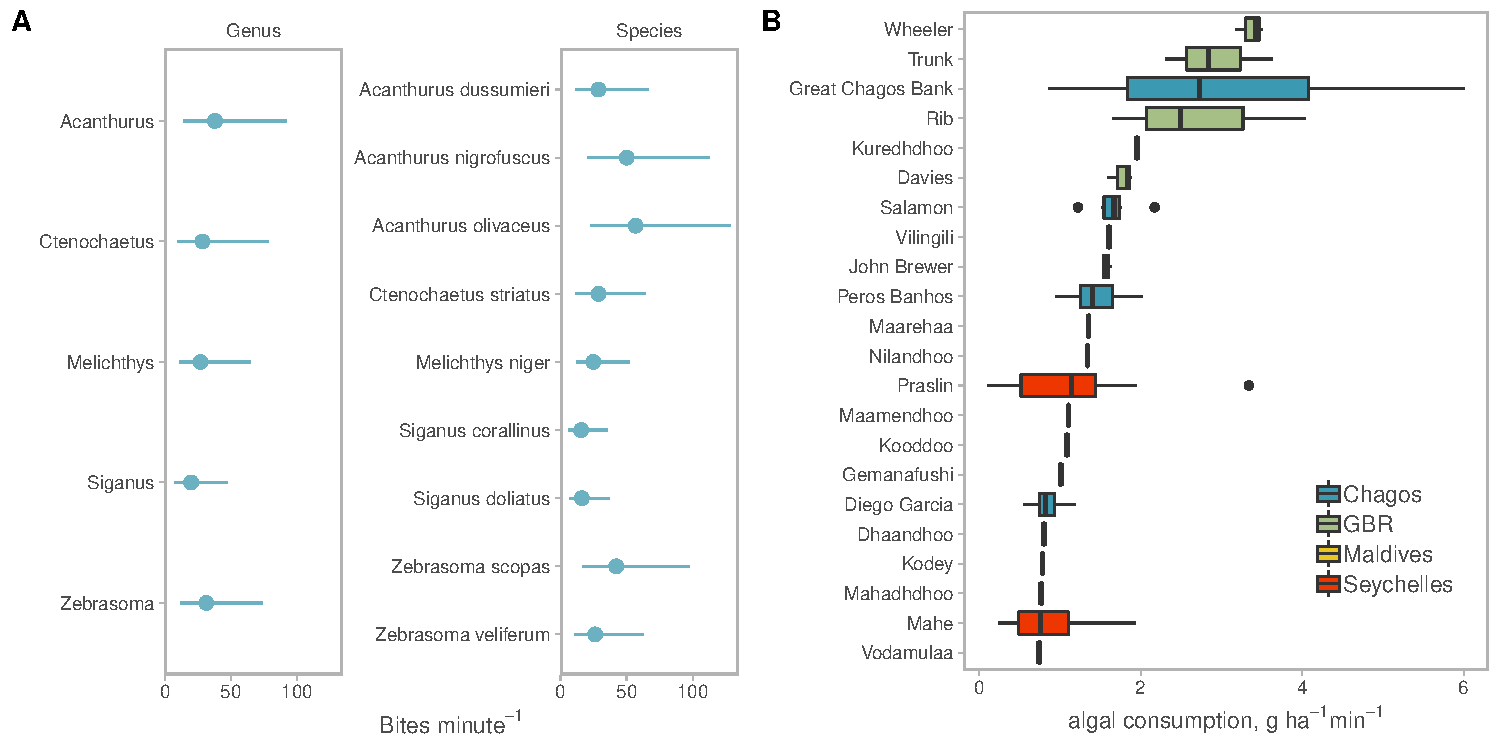
\includegraphics[width=480px]{../../figures/FigureS2_cropper_bites} \end{center}

\textbf{Figure S3 \textbar{} Cropper bite rate predictions (A) and
observed cropper function in UVC (B)} Predicted bite rates are median
posterior predictions with 95\% certainty intervals (A), and boxplots
are site-level observed cropping function for each reef, coloured by UVC
region.

\newpage

\begin{center}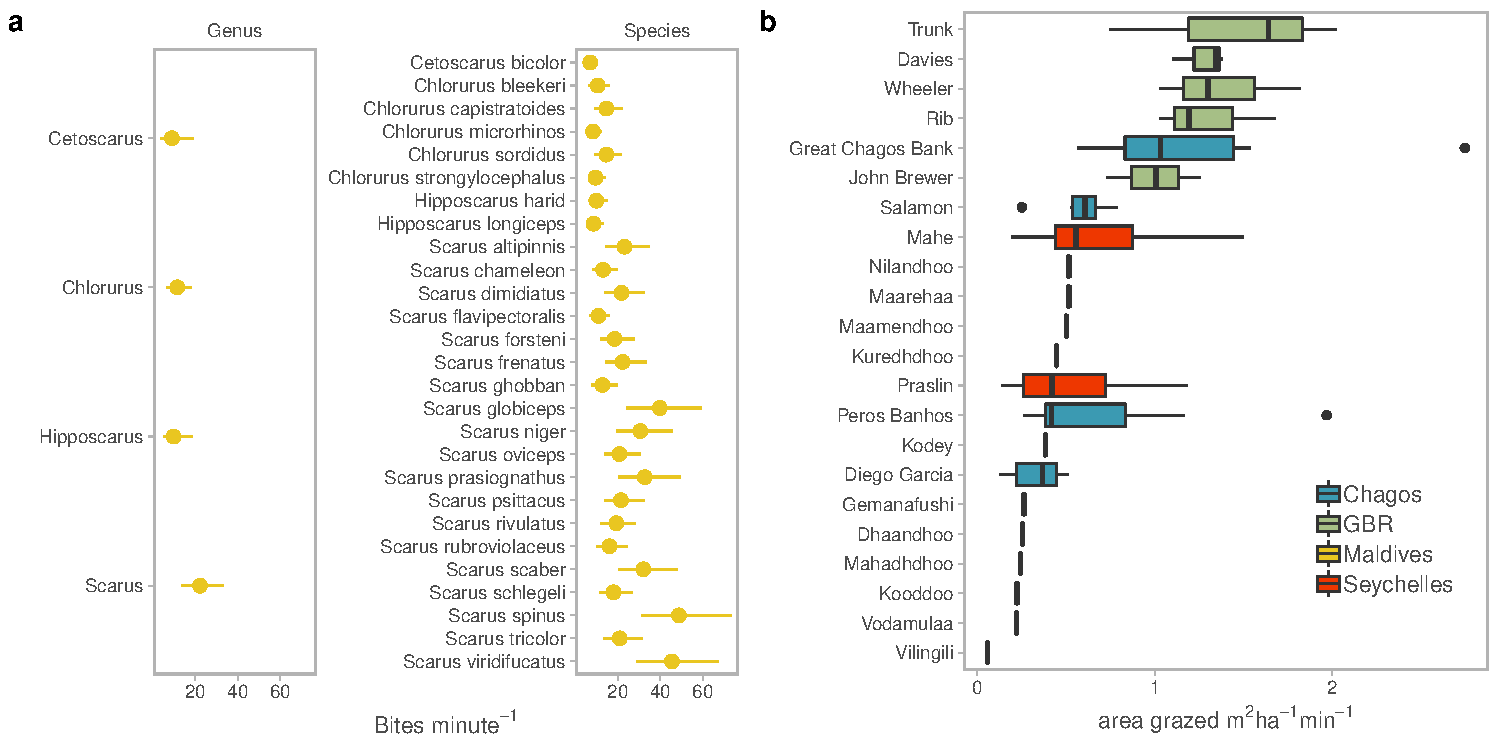
\includegraphics[width=480px]{../../figures/FigureS3_scraper_bites} \end{center}

\textbf{Figure S4 \textbar{} Scraper bite rate predictions (A) and
observed scraping function in UVC (B)} Predicted bite rates are median
posterior predictions with 95\% certainty intervals (A), and boxplots
are site-level observed scraping function for each reef, coloured by UVC
region.

\newpage


\end{document}
